% Created 2015-03-27 Fri 06:21
\documentclass[11pt]{article}
\usepackage[utf8]{inputenc}
\usepackage{lmodern}
\usepackage[T1]{fontenc}
\usepackage{fixltx2e}
\usepackage{graphicx}
\usepackage{longtable}
\usepackage{float}
\usepackage{wrapfig}
\usepackage{rotating}
\usepackage[normalem]{ulem}
\usepackage{amsmath}
\usepackage{textcomp}
\usepackage{marvosym}
\usepackage{wasysym}
\usepackage{amssymb}
\usepackage{amsmath}
\usepackage[version=3]{mhchem}
\usepackage[numbers,super,sort&compress]{natbib}
\usepackage{natmove}
\usepackage{url}
\usepackage{minted}
\usepackage{underscore}
\usepackage[linktocpage,pdfstartview=FitH,colorlinks,
linkcolor=blue,anchorcolor=blue,
citecolor=blue,filecolor=blue,menucolor=blue,urlcolor=blue]{hyperref}
\usepackage{attachfile}
\usepackage[left=1in, right=1in, top=1in, bottom=1in, nohead]{geometry}
\usepackage{fancyhdr}
\usepackage{hyperref}
\usepackage{setspace}
\usepackage[labelfont=bf]{caption}
\usepackage{amsmath}
\usepackage{enumerate}
\usepackage[parfill]{parskip}
\usepackage[version=3]{mhchem}
\author{Prateek Mehta}
\date{\today}
\title{Quantum Chemistry II : HW2}
\begin{document}

\maketitle


\section{A brief note}
\label{sec-1}

The source code and all the files used to create this document is available at \url{https://github.com/prtkm/helium-hartree-fock}.

\section{The code}
\label{sec-2}

Here is the code that perfroms a Hartree Fock simulation for the He atom.

\begin{minted}[frame=lines,fontsize=\scriptsize,linenos]{python}
import numpy as np
from itertools import product
from scipy.linalg import eig


def Suv(z1, z2):
    ''' 
    Returns the overlap terms
    '''
    return (((z1 ** 3) * (z2 ** 3) / np.pi ** 2) ** 0.5) * 2 / (z1 + z2) ** 3 * 4 * np.pi 

def S_matrix(zetas, munus):
    '''
    Returns the overlap matrix
    '''
    S = np.zeros((2,2))
    
    for mu, nu in munus:
        S[mu - 1, nu - 1] =  Suv(zetas[mu], zetas[nu])

    return S   


def Tuv(z1, z2):
    '''
    Returns the kinetic energy integrals
    '''
    return 4 * z1 * z2 * np.sqrt(z1 ** 3 * z2 ** 3 ) / (z1 + z2) ** 3 


def Vuv(z1, z2):
    '''
    Returns the nuclear attraction integrals
    '''
    return - 8 * np.sqrt((z1 ** 3 * z2 ** 3)) / (z1 + z2) ** 2  


def Huv(z1, z2):
    '''
    Returns core hamiltonian elements
    '''
    return Tuv(z1, z2) + Vuv(z1, z2)

def H_matrix(zetas, munus):
    '''
    Returns the core hamiltonian matrix
    '''
    H = np.zeros((2,2))
    
    for mu, nu in munus:
        H[mu - 1, nu - 1] =  Huv(zetas[mu], zetas[nu])

    return H    

def I_two_electron(z):
    '''
    Calculates the two electron integrals
    Args: z = [z1, z2, z3, z4]
    Returns: (z1 z2 | z3 z4)
    '''
    A = np.prod(z) ** 1.5
    
    u = z[0] + z[1]
    v = z[2] + z[3]
    
    integral = 32 * A / u ** 2 * (1 / (u * v ** 2) - 1 / (u + v) ** 3 - 1 / u / (u + v) ** 2)
    return integral


def get_C21(z1, z2, k):

    '''
    Calculates C21
    '''

    S12 = Suv(z1, z2)
    C21 = (1 + k ** 2 + 2 * k * S12) ** -0.5
    return C21
    
def density_matrix(z1, z2, k):
    '''
    Returns the density matrix
    '''

    C21 = get_C21(z1, z2, k)

    P11 = 2 * C21 ** 2 * k ** 2
    P12 = 2 * k * C21 ** 2 
    P21 = P12
    P22 = 2 * C21 ** 2    
    P =  np.array([[P11, P12],
                   [P21, P22]])
    return P


def G_matrix(zetas, k, munus, lambdasigmas):

    '''
    Returns the G Matrix
    '''
    
    G = np.zeros((2,2))

    P = density_matrix(zetas[1], zetas[2], k)
                       
    for mu, nu in munus:    

        g = 0
        for l, s in lambdasigmas:

            int1 = I_two_electron((zetas[mu], zetas[nu], zetas[s], zetas[l]))
            int2 = I_two_electron((zetas[mu] , zetas[l], zetas[s], zetas[nu]))
  
            g+= P[l - 1, s - 1] * (int1 - 0.5 * int2)

        G[mu - 1, nu - 1] = g
    return G


def F_matrix(zetas, k, munus, lambdasigmas):
    '''
    Returns the Fock matrix
    '''
    return H_matrix(zetas, munus) + G_matrix(zetas, k, munus, lambdasigmas)


def secular_eqn(F, S):
    '''
    Returns the eigen values and eigen vectors of the secular eqn
    '''    
    ei, C = eig(F, S)
    return ei, C


def get_E0(P, H, F, orb_nos):

    '''
    Returns the hartree-fock energy
    '''
    
    E0 =0
    for mu in orb_nos:

        for nu in orb_nos:
            E0 += 0.5 * (P[mu -1, nu - 1] * (H[mu - 1, nu - 1] + F[mu - 1, nu - 1]))

    return E0

def calculate(z1, z2, k):
    '''
    Calculate HF energy, k, C11, C12
    '''
    
    orb_nos = [1,2]

    # Store zetas in a dictionary    
    zetas = {1:z1, 2:z2}

    # mu-nu combinations
    munus = list(product(orb_nos,repeat=2))
    
    # lambda-sigma combinations
    lambdasigmas =  list(product(orb_nos,repeat=2))
    
    # Calculate overlap integrals
    S = S_matrix(zetas, munus)

    # Calculate core hamiltonian
    H = H_matrix(zetas, munus)
    
    # Calculate density_matrix
    P = density_matrix(z1, z2, k)
    
    # Calculate Fock Matrix
    F = F_matrix(zetas, k, munus, lambdasigmas)

    # Solve secular eqn
    ei, C = secular_eqn(F, S)

    # get k
    k = C[0, 0] / C[1, 0]

    # Calculate HF energy
    E0 = get_E0(P, H, F, orb_nos)

    return E0, k, C[0,0], C[1,0]
     
def main(*args):
    '''
    Takes zeta1, zeta2, k, and max convergence steps as input and performs a 
    scf calculation on the helium atom.
    '''

    from argparse import ArgumentParser

    parser = ArgumentParser(description='Helium Hartree Fock')
    parser.add_argument('-z1', type=float, help="zeta 1", default=1.45)
    parser.add_argument('-z2', type=float, help="zeta2", default=2.91)
    parser.add_argument('-k0', type=float, help="k = C11 / C21", default=2.)      
    parser.add_argument('-n', default=20, type=int,
                        help='Max. number of scf steps')

    args = parser.parse_args()

    z1 = args.z1
    z2 = args.z2
    k0 = args.k0
    n = args.n
    
    k = k0
    C21_0 = get_C21(z1, z2, k)    
    C11_0 = k0 * C21_0
    
    print '-' * 20
    print 'Starting Simulation'
    print '-' * 20
    print '\nInitial Parameters:'
    print 'z1 = {0}, z2 = {1}, k = {2}\n'.format(z1, z2, k0)

    for i in range(n):

        print '-' * 20
        print 'Entering Iteration {0}'.format(i + 1)
        print '-' * 20
        
        print 'Using k = {0}\n'.format(k)

        E0, k, C11, C21 = calculate(z1, z2, k)
        
        print 'Iteration results:'
        print 'E0 = {E0}\nk = {k}\nC11 = {C11}\nC21 ={C21}\n'.format(**locals())
        print 'Convergence level:'
        print 'dC11 = {0:1.5f}'.format(np.abs(C11 - C11_0))
        print 'dC21 = {0:1.5f}\n'.format(np.abs(C21 - C21_0))

        if (np.abs(C11 - C11_0) < 1e-4) and (np.abs(C21 - C21_0) < 1e-4):
            print '\nReached required accuracy in {0} iterations. Stopping Simulation.'.format(i+1)
            print '-' * 20
            converged = True
            break

        else:
            C11_0 = C11
            C21_0 = C21
            
    return

if __name__ == '__main__':
    import sys
    main(*sys.argv)
\end{minted}


\section{A demo}
\label{sec-3}

Here is an example of running the code from the command line.

\begin{minted}[frame=lines,fontsize=\scriptsize,linenos]{sh}
python helium-hf.py -z1 1.45 -z2 2.91 -k 2
\end{minted}

\begin{verbatim}
--------------------
Starting Simulation
--------------------

Initial Parameters:
z1 = 1.45, z2 = 2.91, k = 2.0

--------------------
Entering Iteration 1
--------------------
Using k = 2.0

Iteration results:
E0 = -2.80340885254
k = 4.39285140431
C11 = -0.975054861762
C21 =-0.221963998328

Convergence level:
dC11 = 1.66733
dC21 = 0.56810

--------------------
Entering Iteration 2
--------------------
Using k = 4.39285140431

Iteration results:
E0 = -2.86154894126
k = 4.59847490385
C11 = -0.977161737138
C21 =-0.212496916384

Convergence level:
dC11 = 0.00211
dC21 = 0.00947

--------------------
Entering Iteration 3
--------------------
Using k = 4.59847490385

Iteration results:
E0 = -2.86166925837
k = 4.60894179682
C11 = -0.97726184348
C21 =-0.212036056553

Convergence level:
dC11 = 0.00010
dC21 = 0.00046

--------------------
Entering Iteration 4
--------------------
Using k = 4.60894179682

Iteration results:
E0 = -2.86166954612
k = 4.60945632151
C11 = -0.977266747654
C21 =-0.212013452236

Convergence level:
dC11 = 0.00000
dC21 = 0.00002


Reached required accuracy in 4 iterations. Stopping Simulation.
--------------------
\end{verbatim}



\section{Number of iterations required}
\label{sec-4}

The script below dumps out the energies for each scf step and the number of iterations required to reach scf convergence. It appears that for almost every initial guess of k, it takes about 4 iterations to reach convergence. The final energy converges to the same value, so everything looks ok.

\begin{minted}[frame=lines,fontsize=\scriptsize,linenos]{sh}
for k in 100 10 1 0 -1 -10 -100
do
    echo 'k =' $k':'
    python helium-hf.py -z1 1.45 -z2 2.91 -k $k | grep E0
    python helium-hf.py -z1 1.45 -z2 2.91 -k $k | grep iterations
    echo
done
\end{minted}

\begin{verbatim}
k = 100:
E0 = -2.79861910194
E0 = -2.86149366533
E0 = -2.86166911997
E0 = -2.86166954579
Reached required accuracy in 4 iterations. Stopping Simulation.

k = 10:
E0 = -2.84420725495
E0 = -2.86162407309
E0 = -2.86166943689
E0 = -2.86166954655
Reached required accuracy in 4 iterations. Stopping Simulation.

k = 1:
E0 = -2.60762540507
E0 = -2.86123079718
E0 = -2.86166850379
E0 = -2.86166954431
Reached required accuracy in 4 iterations. Stopping Simulation.

k = 0:
E0 = -1.35315
E0 = -2.86038789542
E0 = -2.86166652738
E0 = -2.86166953956
Reached required accuracy in 4 iterations. Stopping Simulation.

k = -1:
E0 = 2.95510515363
E0 = -2.83075943672
E0 = -2.86158698026
E0 = -2.86166934694
E0 = -2.86166954634
Reached required accuracy in 5 iterations. Stopping Simulation.

k = -10:
E0 = -2.68444788097
E0 = -2.86112538719
E0 = -2.86166821819
E0 = -2.86166954362
Reached required accuracy in 4 iterations. Stopping Simulation.

k = -100:
E0 = -2.78334855542
E0 = -2.8614474518
E0 = -2.86166900728
E0 = -2.86166954552
Reached required accuracy in 4 iterations. Stopping Simulation.
\end{verbatim}


\section{Checking with 'Optimal Values'}
\label{sec-5}

Here is the test to calculate with the reported optimal values of $\zeta$$_{\text{1}}$ and $\zeta$$_{\text{2}}$. It looks like it perfectly matches the value reported by Roetti and CLementi.

\begin{minted}[frame=lines,fontsize=\scriptsize,linenos]{sh}
python helium-hf.py -z1 1.45363 -z2 2.91093 -k 4.60 | tail -15 | grep E0
\end{minted}

\begin{verbatim}
E0 = -2.86167259768
\end{verbatim}


\section{Energy as a function of $\zeta$$_{\text{1}}$}
\label{sec-6}

Plotting over a range of values of $\zeta$$_{\text{1}}$, at the optimal $\zeta$$_{\text{2}}$ value, we find that the reported $\zeta$$_{\text{1}}$ value gives the lowest energy.

\begin{minted}[frame=lines,fontsize=\scriptsize,linenos]{python}
from subprocess import Popen, PIPE
import numpy as np
import matplotlib.pyplot as plt

z1s = np.linspace(1.45363*0.9, 1.45363*1.10, 11)
energies = []

for z1 in z1s:
    
    cmd = 'python helium-hf.py -z1 {0} -z2 2.91093 -k 2'.format(z1)
    p = Popen(cmd.split(), stdout=PIPE, stdin=PIPE, stderr=PIPE)
    
    out, err = p.communicate()
    
    # parse output file
    for line in out.split('\n'):
         if 'E0' in line: 
            E0 = float(line.split()[-1])

    energies.append(E0)
    
plt.plot(z1s, energies, 'bo-', lw=2, ms=10)
plt.ticklabel_format(useOffset=False)
plt.xlabel('$\zeta_{1}$', fontsize=24)
plt.ylabel('Energy (a.u.)', fontsize=24)
plt.tight_layout()
plt.savefig('optimal-zeta-1.png')
plt.show()
\end{minted}

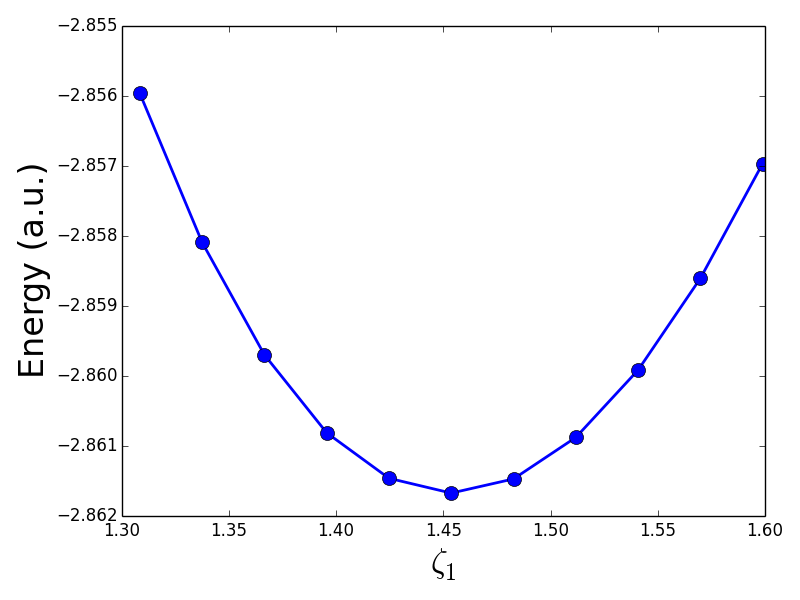
\includegraphics[width=.9\linewidth]{./optimal-zeta-1.png}
% Emacs 24.4.1 (Org mode 8.2.10)
\end{document}